\section{Deep Sequential Models}
\subsection{Autoregressive Models}
\begin{itemize}
	\item Generative models without latent variables, but assuming an order in the data (if there is no, create an artificial order like image from left to right, top to bottom). The likelihood is the product of conditionals:
	$$p(x)=\prod_{k=1}^{D} p(x_k|x_{j<k})$$
	\item In contrast to RNNs, there is no/not necessarily parameter sharing, and the chain cannot be of infinite length because of that
	\item \textit{Advantages}: $p(x)$ is tractable
	\item \textit{Drawbacks}: training and generation is slow due to being sequential and not parallel
\end{itemize}
\subsubsection{NADE}
\begin{itemize}
	\item Originally defined for binary inputs/data. Can be generalized for other spaces as well
	\item Every output $x_d$ is modeled by a single layer that takes as input all previous data points, and generates based on that it's prediction:
	\begin{equation*}
		\begin{split}
			p(x_d=1|x_{<d}) & = \sigma\left(V_{d,:}\cdot h_d + b_d\right), h_d = \sigma\left(W_{:,<d}\cdot x_{<d} + c\right)
		\end{split}
	\end{equation*}
	where $V\in \mathbb{R}^{D\times H}, W\in \mathbb{R}^{H\times D}, b\in \mathbb{R}^{D}, c\in \mathbb{R}^{H}$ ($H$ hidden dimensionality, $D$ input dimensions)
	\item Objective is minimizing log likelihood: $\mathcal{L} = - \log p(x) = - \sum_{k=1}^{D} p(x_k|x_{<k})$
	\begin{figure}[ht!]
		\centering
		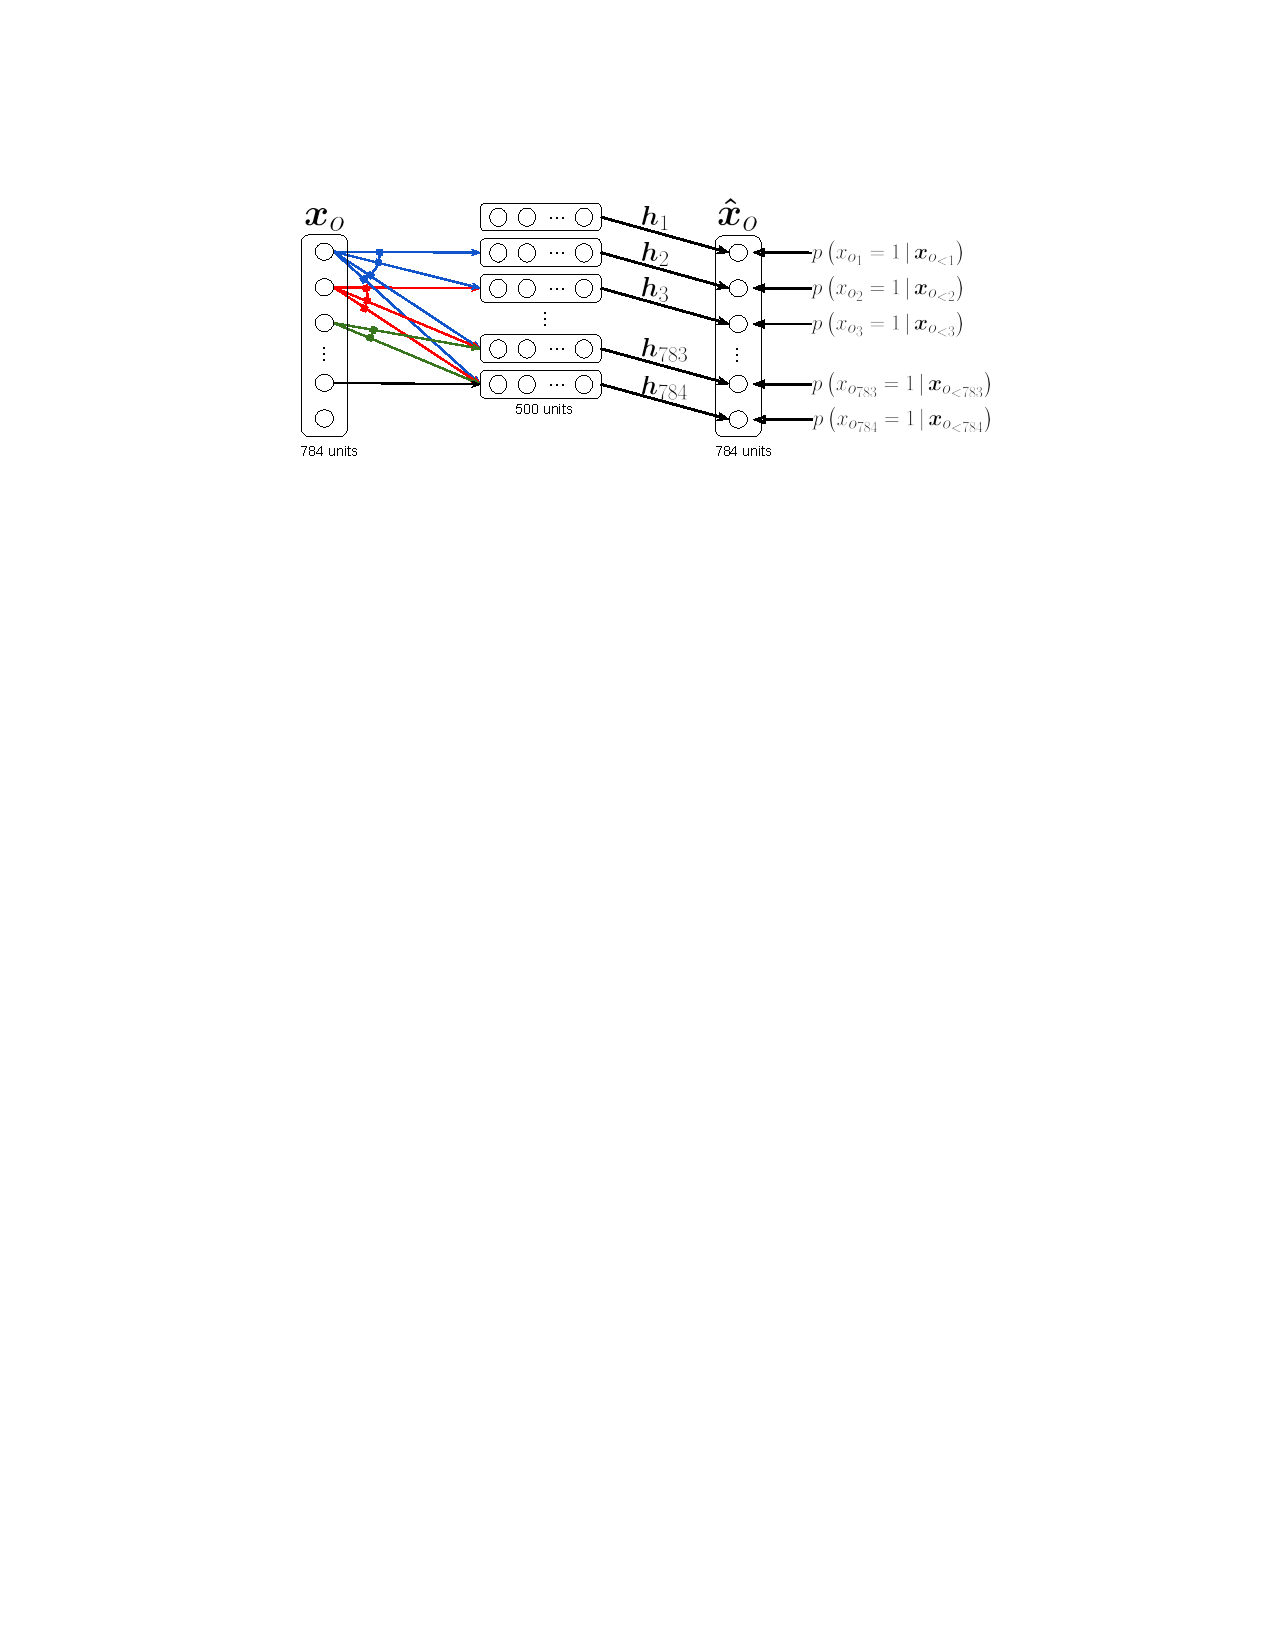
\includegraphics[width=0.6\textwidth]{figures/Autoregressive_NADE.pdf}
		\caption{Concept of NADE.}
	\end{figure}
	\item \textit{Teacher forcing}: During training, use ground truth as input for all levels. For testing, use generated samples as input (sequentially)
\end{itemize}
\subsubsection{MADE}
\begin{itemize}
	\item Use an autoencoder where we carefully mask out connections so that the output $y_d$ only depends on inputs $x_{<d}$
	\item Name ``autoencoder'' is only because we try to reproduce the input. However, note that we neither have a bottleneck nor we try to get sparsity. We just remove connections to make the outputs depending on certain inputs
	\begin{figure}[ht!]
		\centering
		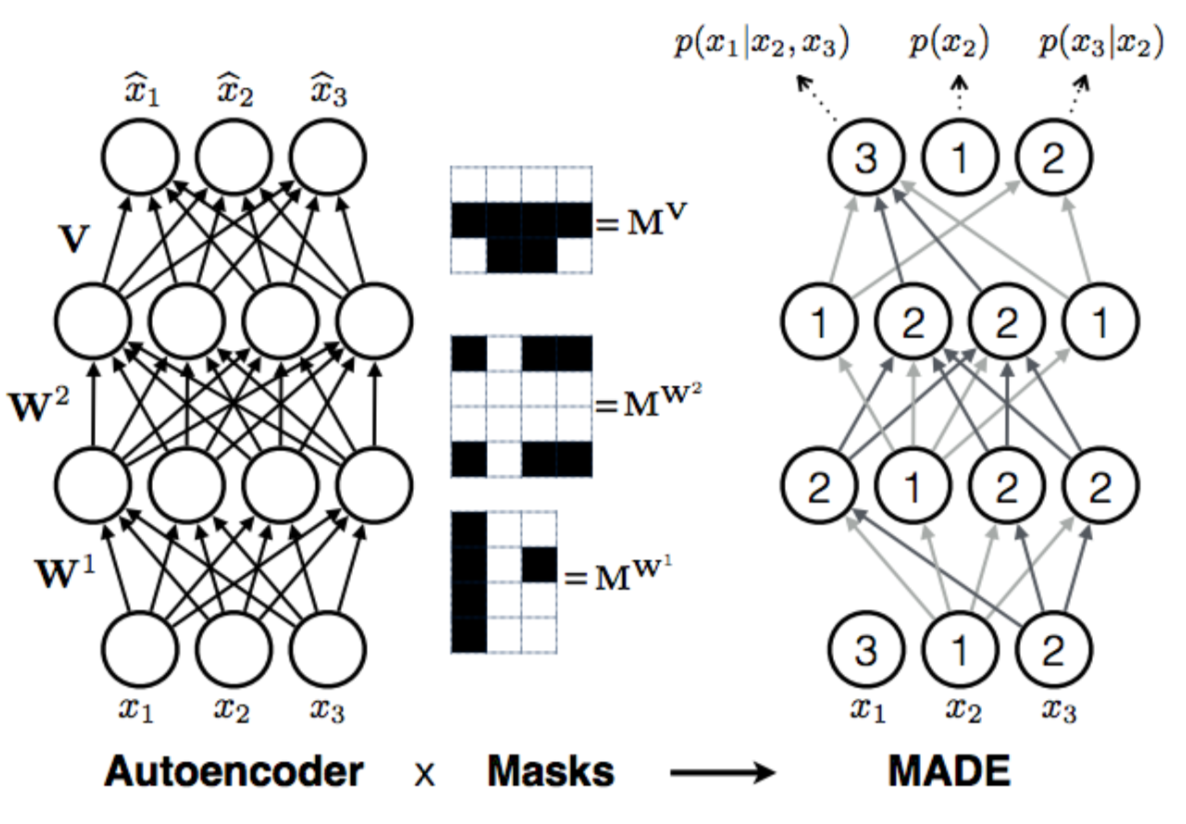
\includegraphics[width=0.4\textwidth]{figures/Autoregressive_MADE.png}
		\caption{Masked autoencoder for autoregressive models. We set certain weights to 0 (i.e. remove connections between neurons) so that the generation of $x_1$ only depends on $x_2$ and $x_3$, but not on $x_1$ itself (which would be cheating and prevent the model of being generative).}
	\end{figure}
\end{itemize}
\subsubsection{PixelRNN}
\begin{itemize}
	\item Assume row-wise pixel and sequential color generation (first red channel, then green, afterwards blue):
	$$p(x_i|x_{<i}) = p(x_{i,R}|x_{<i})\cdot p(x_{i,G}|x_{i,R}, x_{<i})\cdot p(x_{i,B}|x_{i,R}, x_{i,G}, x_{<i})$$
	\item Different ways of modeling it. LSTM variants mostly have 12 layers
	\begin{itemize}
		\item \textit{Row LSTM}: to compute next output (i.e. next hidden state), we take into consideration the three hidden states of the row above a certain pixel as ``last hidden state''. We get therefore a tri-angular shape of context. However, it thereby misses context from the row itself, and further away context. As it does not use pixels in the same row, the computation can be parallelized for a row. 
		\item \textit{Diagonal Bi-LSTM}: Uses all pixels that were generated before by using a Bi-LSTM. 
	\end{itemize}
	\begin{figure}[ht!]
		\centering
		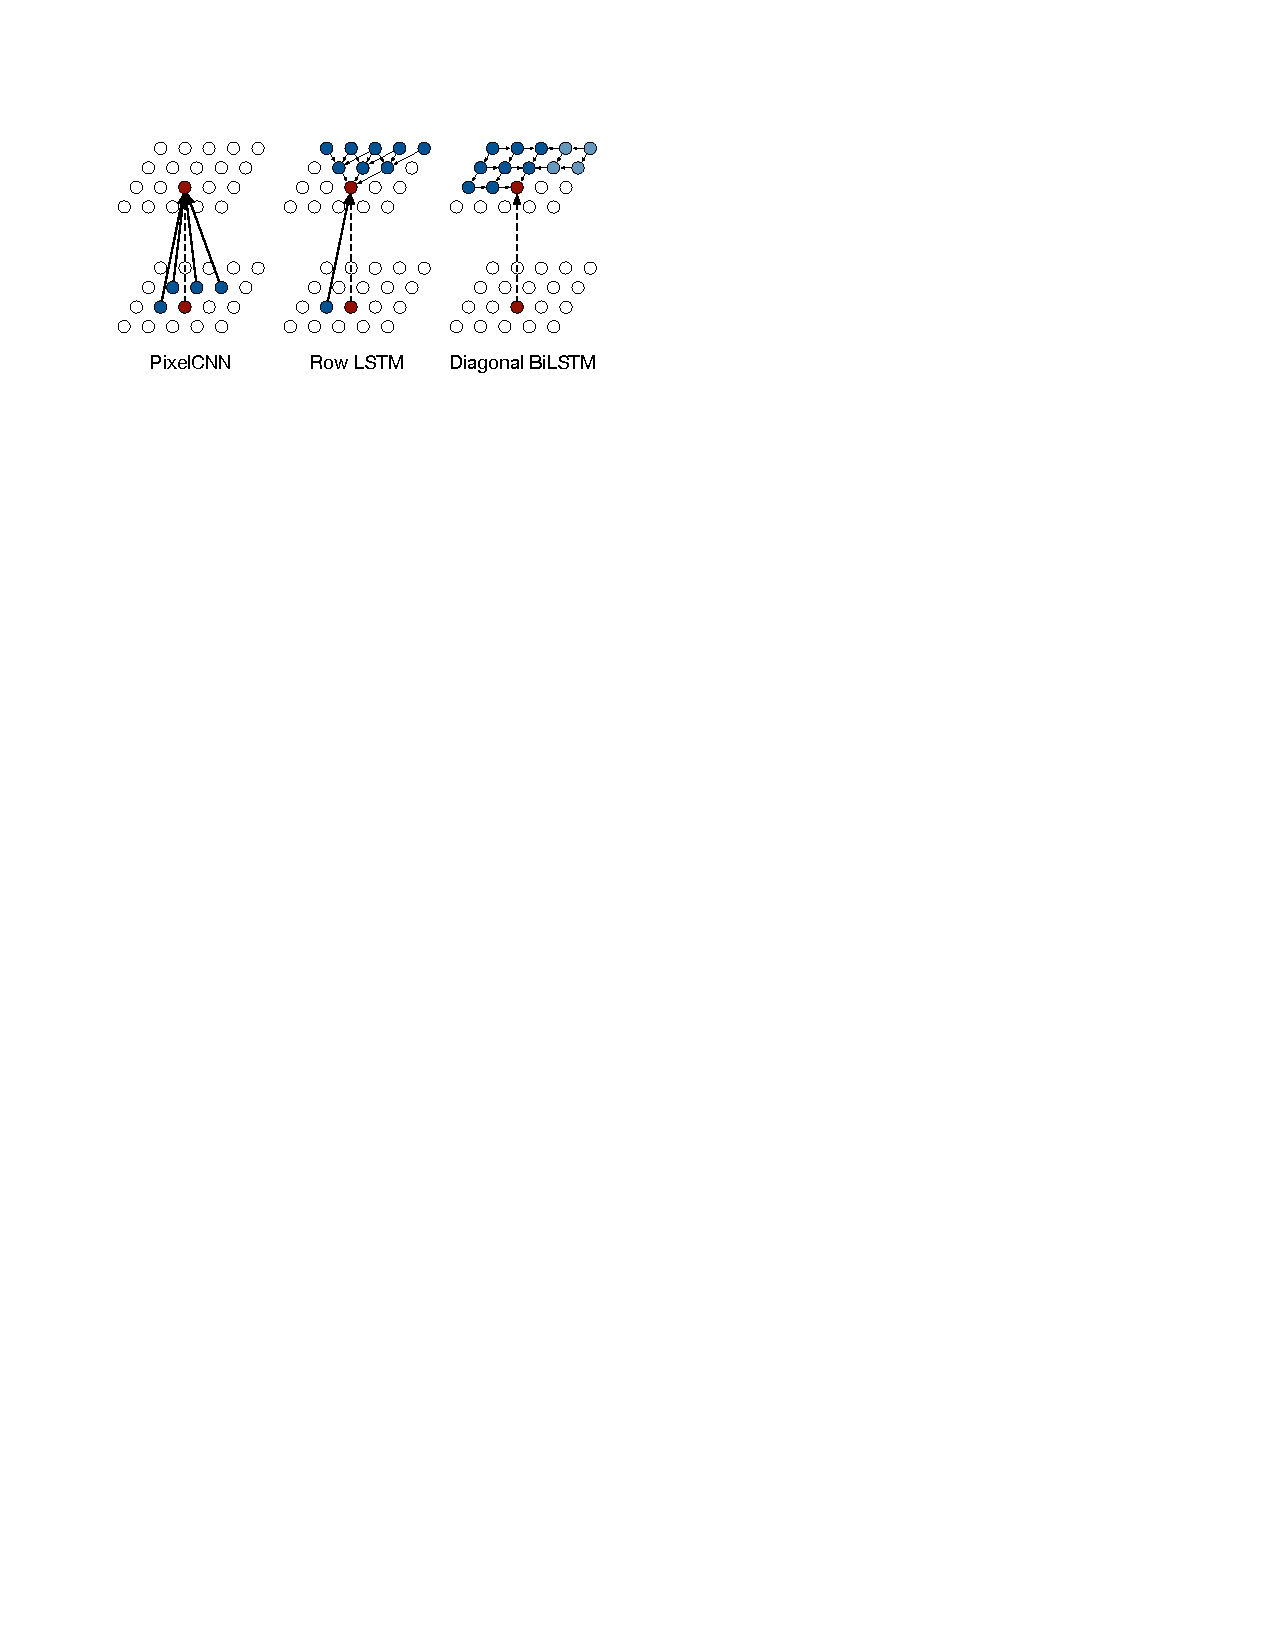
\includegraphics[width=0.4\textwidth]{figures/Autoregressive_PixelRNN.pdf}
		\caption{Comparing different methods of PixelRNN and PixelCNN. The lower level is the previous layer, and the top is the next layer. If we have a single layer PixelRNN/CNN, the lower one would be the input and the upper the generated output.}
		\label{fig:Autoregressive_PixelRNN}
	\end{figure}
	\item The architecture includes residual connections to speed up training
	\item \textit{Benefits}: good modeling of $p(x)$, reasonable image quality
	\item \textit{Disadvantages}: slow training and slow generation
\end{itemize}
\subsubsection{PixelCNN}
\begin{itemize}
	\item Replace recurrence by convolutions to speed up (at least) training
	\item Convolutions are masked so that only context from before (i.e. left and top) can be used. See Figure~\ref{fig:Autoregressive_PixelRNN} left and Figure~\ref{fig:Autoregressive_PixelCNN} for an example
	\begin{figure}[ht!]
		\centering
		\begin{subfigure}{0.3\textwidth}
			\centering
			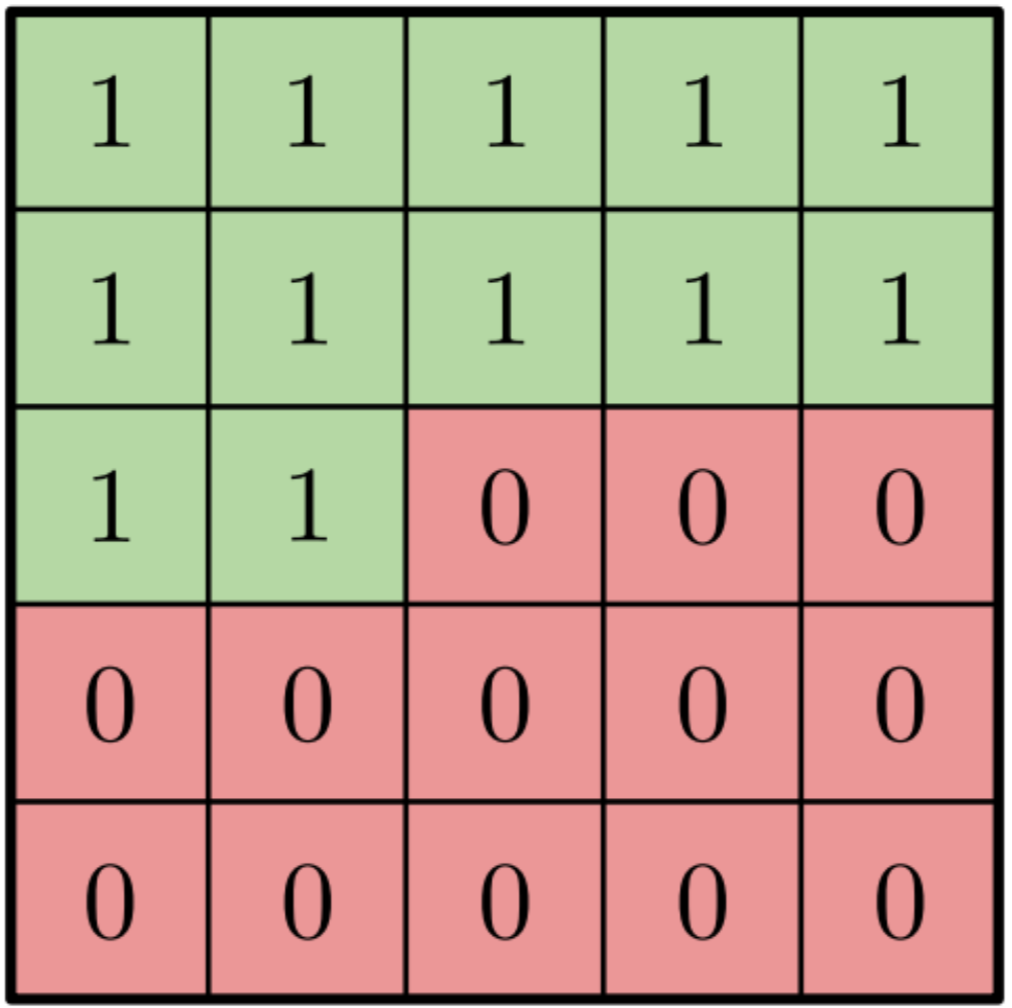
\includegraphics[width=0.6\textwidth]{figures/Autoregressive_Masked_Conv.png}
			\caption{Example mask for $5\times 5$ convolution}
		\end{subfigure}
		\hspace{2mm}
		\begin{subfigure}{0.32\textwidth}
			\centering
			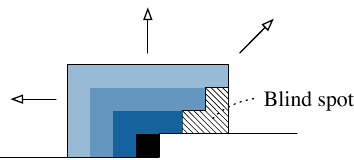
\includegraphics[width=\textwidth]{figures/Autoregressive_PixelCNN_blindspot_problem.png}
			\caption{Blindspot of PixelCNN}
		\end{subfigure}
		\hspace{2mm}
		\begin{subfigure}{0.32\textwidth}
			\centering
			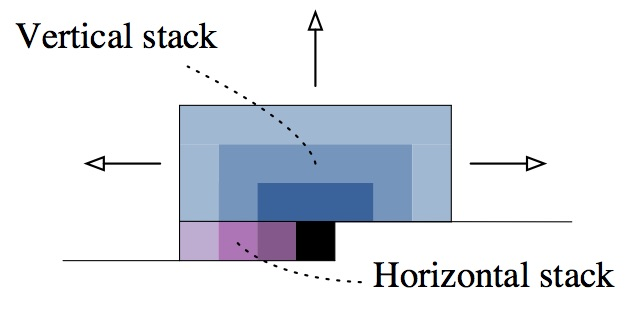
\includegraphics[width=\textwidth]{figures/Autoregressive_PixelCNN_blindspot.jpg}
			\caption{Solution to blindspot}
		\end{subfigure}
		\caption{Masked convolutions in PixelCNN}
		\label{fig:Autoregressive_PixelCNN}
	\end{figure}
	\item Problem: worse results than PixelRNN because of limited context and blind spot (cascaded convolutions ignore right upper part)
	\item Solution: use two convolutions, one vertical stack looking purely on the top part, and the horizontal stack looking to the right. Additionally, use gated convolutions (one half of the features go through tanh, the other through sigmoid)
	\item \textbf{PixelCNN++}: replace softmax with logistic mixture likelihood over 8 bits, use encoder-decoder architecture with skip connections
\end{itemize}
\subsubsection{PixelVAE}
\begin{itemize}
	\item Standard VAE with PixelCNN as decoder/generator
	\item However, generator is very powerful which can lead to the problem that it ignores the latent code, and just generates ``nice'' images
	\begin{figure}[ht!]
		\centering
		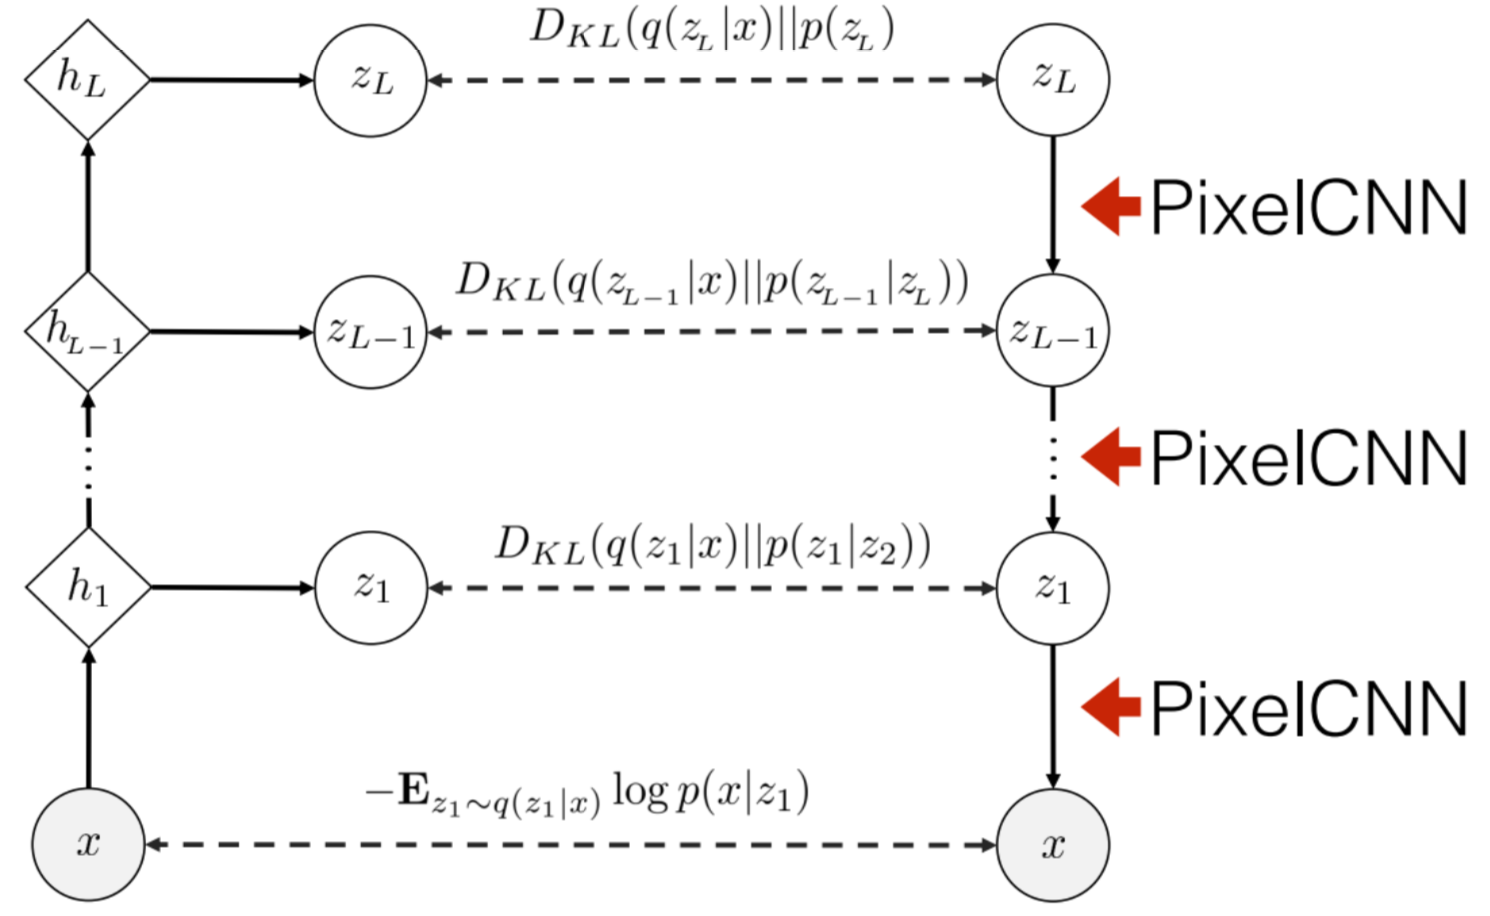
\includegraphics[width=0.3\textwidth]{figures/Autoregressive_PixelVAE.png}
		\caption{Architecture of a PixelVAE}
	\end{figure}
\end{itemize}